\section{Theoretical Analysis}
\label{sec:analysis}

In this section, we used a suitable theoretical model that was able to estimate the  circuit behavior in response to frequency.

\subsection{Ideal OPAMP analysis}

In this subsection we used the characteristics of an ideal OPAMP to determine the behavior of the circuit. We considered:

\begin{equation}
   \frac{v_0}{v_I} = - \frac{R_2}{R_1} 
\end{equation}
\begin{equation}
   Z_I = R_\infty
\end{equation}
\begin{equation}
   Z_O = 0
\end{equation}

\subsubsection{Circuit Transfer Function}

By determining the above-referenced parameters, we were able to compute the transfer function of our ideal circuit:

\begin{equation}
   \frac{v_o(s)}{v_i(s)} =\left(1 + \frac{R3}{R2}\right) \times \frac{R1 \times C1 \times s}{1 + (R1 \times C1 \times s)}
\end{equation}

With the frequency response as follows: 

\begin{figure}[H] \centering
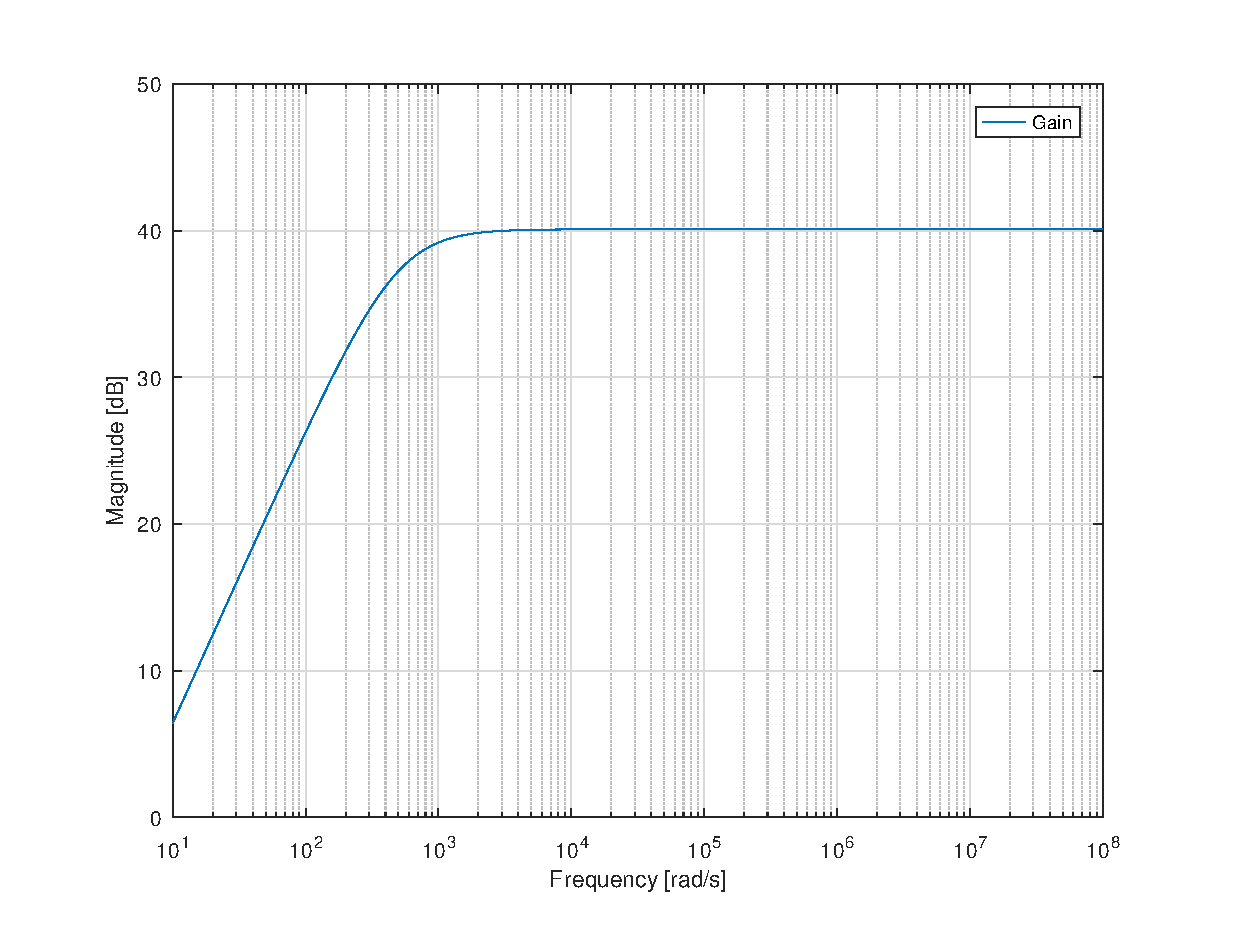
\includegraphics[width=0.8\linewidth]{b1.eps}
\caption{Gain stage circuit (from lecture 17 TCFE) }
\label{fig:rc2}
\end{figure} 

\begin{figure}[H] \centering
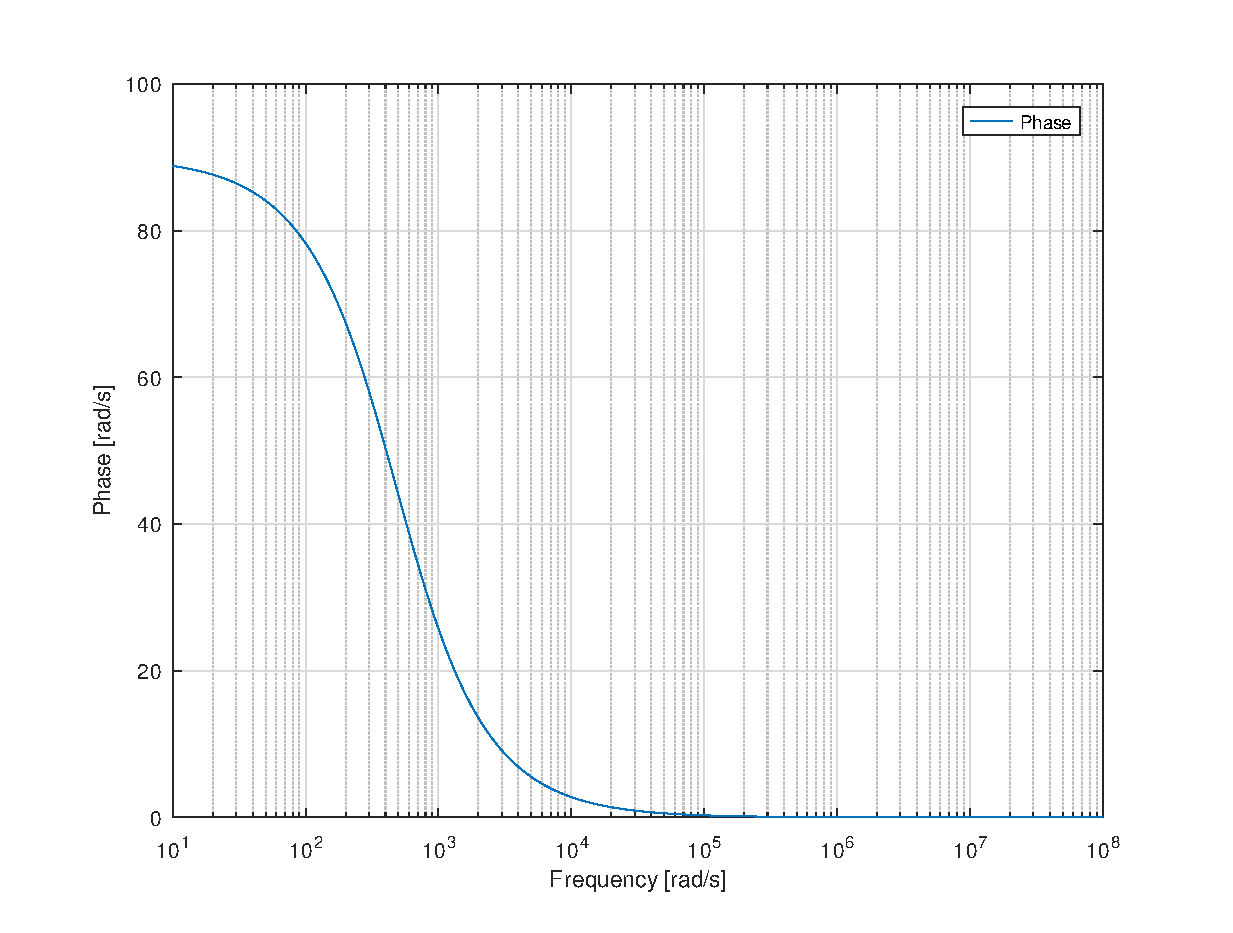
\includegraphics[width=0.8\linewidth]{b2.eps}
\caption{Gain stage circuit (from lecture 17 TCFE) }
\label{fig:rc2}
\end{figure} 

As we can see, the ideal behavior of the OPAMP does not equals the simulated behavior. This is because, the ideal behavior does not take into account that the OPAMP has two poles, which end up making the response to be a Band-Pass and not just an high pass. having said that, we had to use a more adequate model for its theoretical analysis. 

\vspace{-1cm}
\subsection{Circuit analysis}

For a more adequate analysis, and taking into account the non-ideal behavior of OPAMP, we implemented a circuit in order to be able to predict the location of the poles of the OPAMP transfer function. Thus, we verified that the OPAMP has two poles, one at $10^4$ and the other at $10^6$. It was possible to perceive this through the magnitude and phase Bode plots. As you can see, the slope changes in $10^4$ to -20 dB per decade, and in $10^6$ to -40 dB per decade.


\begin{figure}[H]
  \centering
  \begin{minipage}[b]{0.45\textwidth}
    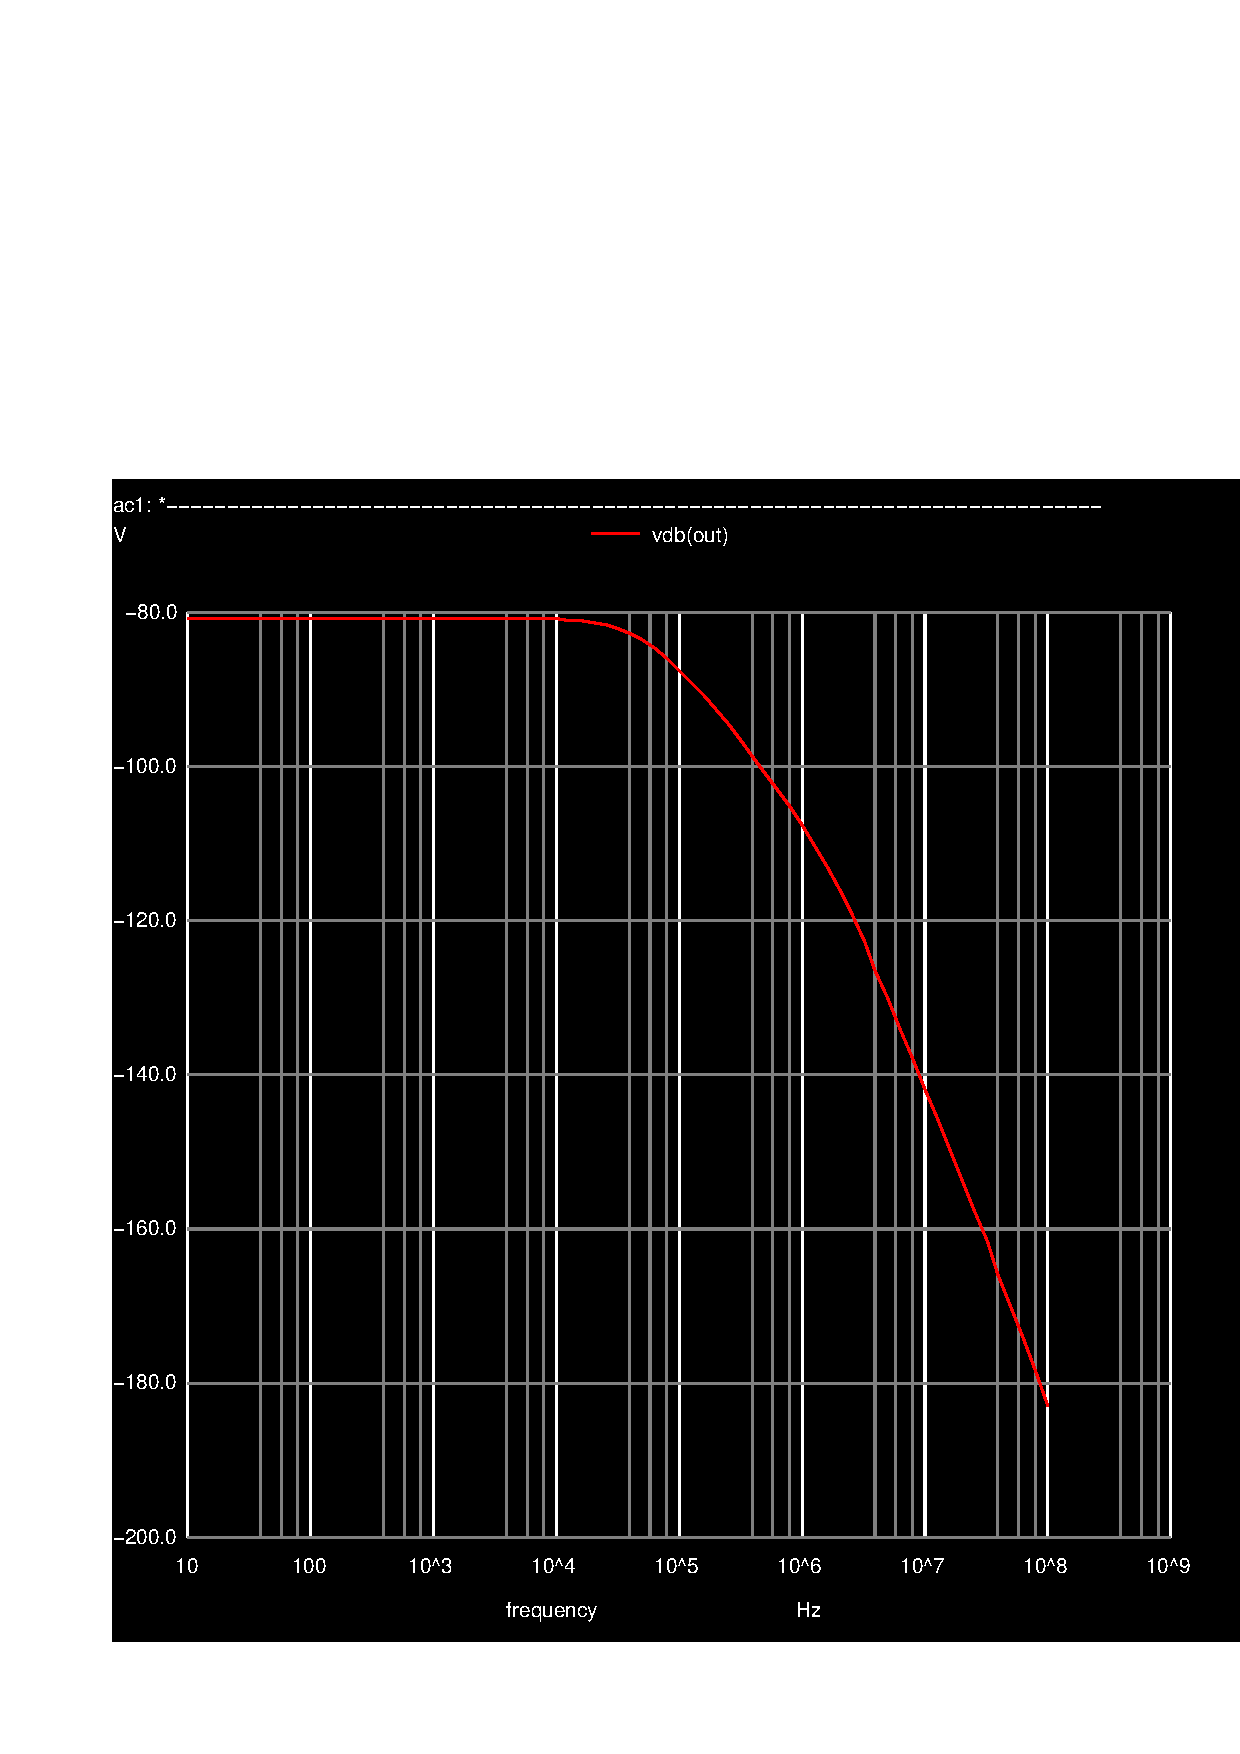
\includegraphics [scale=0.3]{opampdb.pdf}
    \caption{OPAMP frequency response: magnitude}
    \label{fig:my_label}
  \end{minipage}
  \hfill
  \begin{minipage}[b]{0.45\textwidth}
    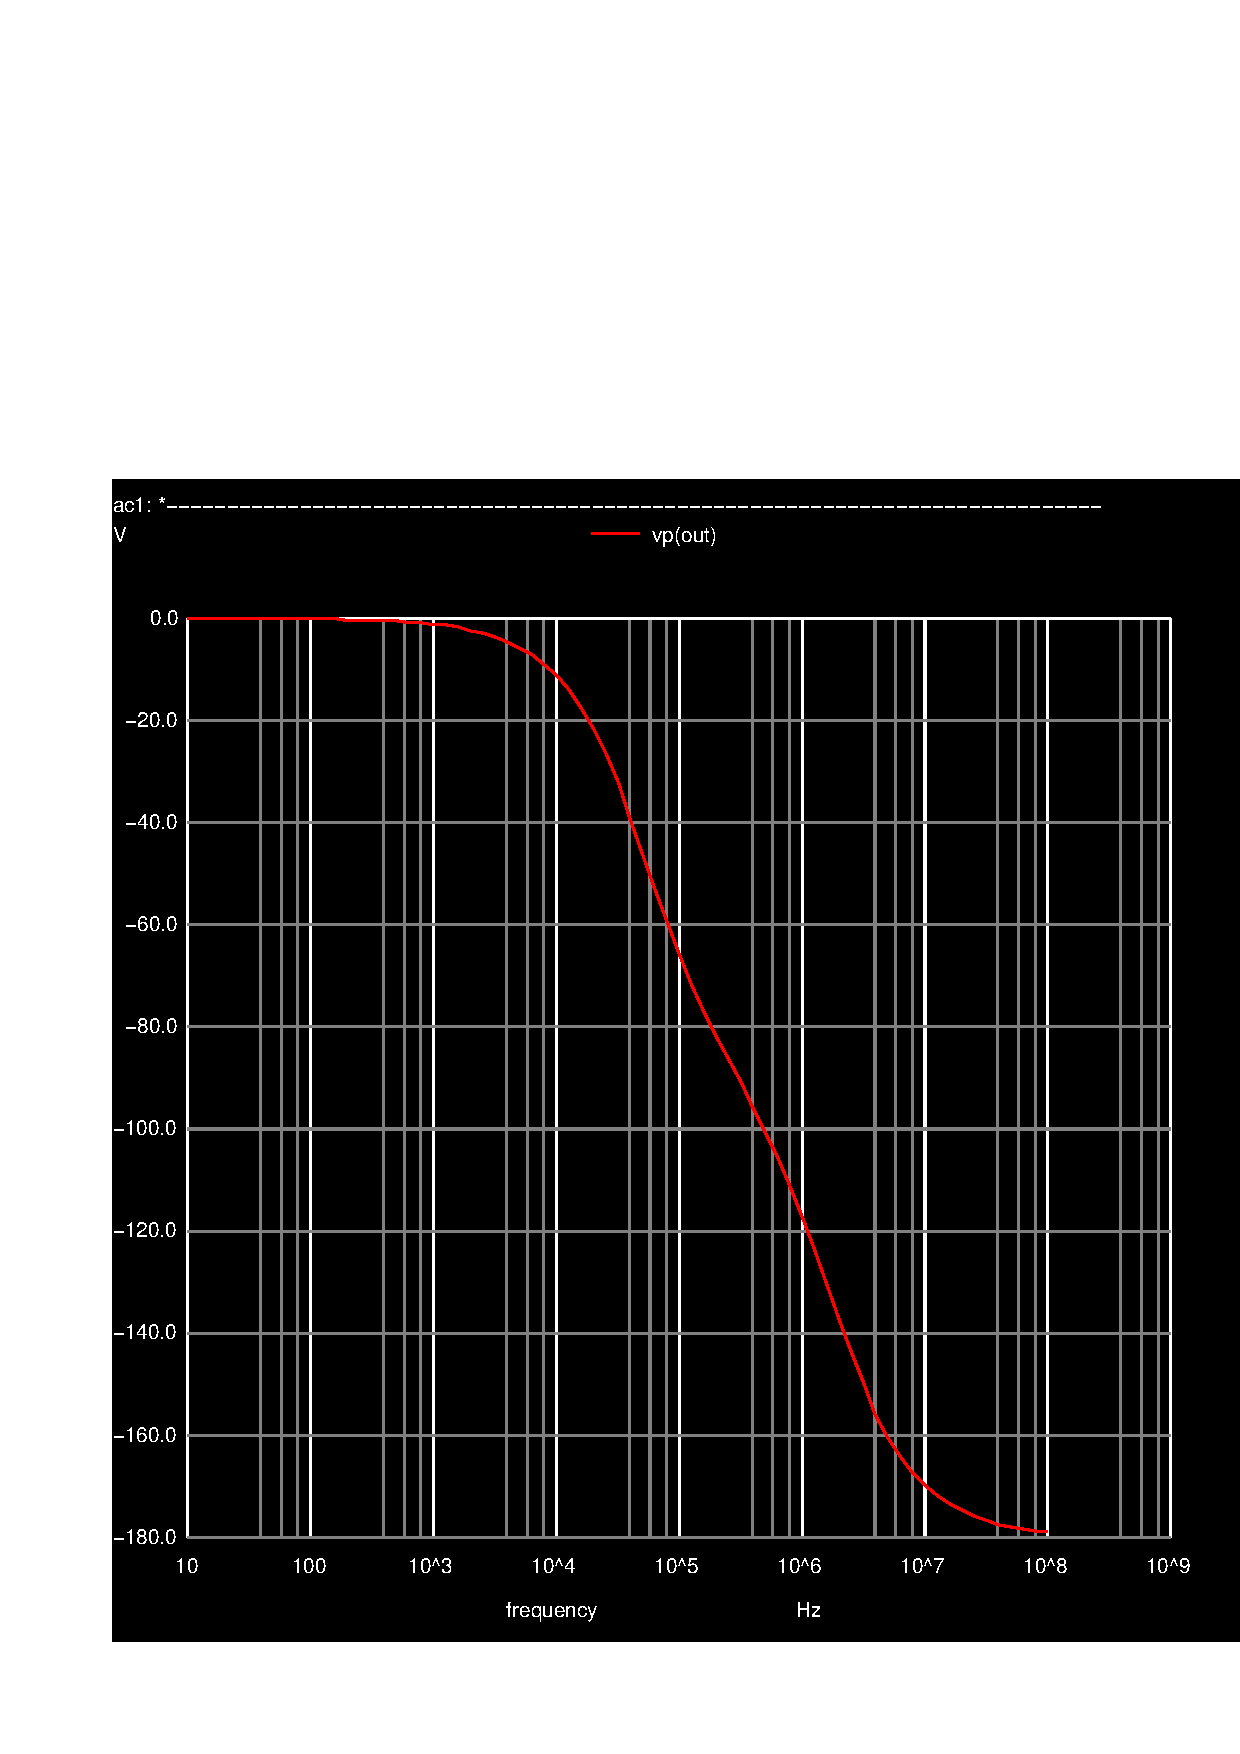
\includegraphics [scale=0.3] {opampp.pdf}
    \caption{OPAMP frequency response: phase}
    \label{fig:my_label}
  \end{minipage}
\end{figure}



\subsubsection{Circuit Transfer Function}

In this way, it was possible to correct the previously computed transfer function in order to incorporate the non-ideal behavior of OPAMP. The obtained FT is: 

\begin{equation}
    \frac{v_o(s)}{v_i(s)} = 1 + (\frac{R3}{R2}) \times \frac{R1 \times C1 \times s}{1 + (R1 \times C1 \times s)} \times \frac{10 e10}{(s + 10 e6) \times (s+10 e4)}
\end{equation}

And the response is:

\begin{figure}[H] \centering
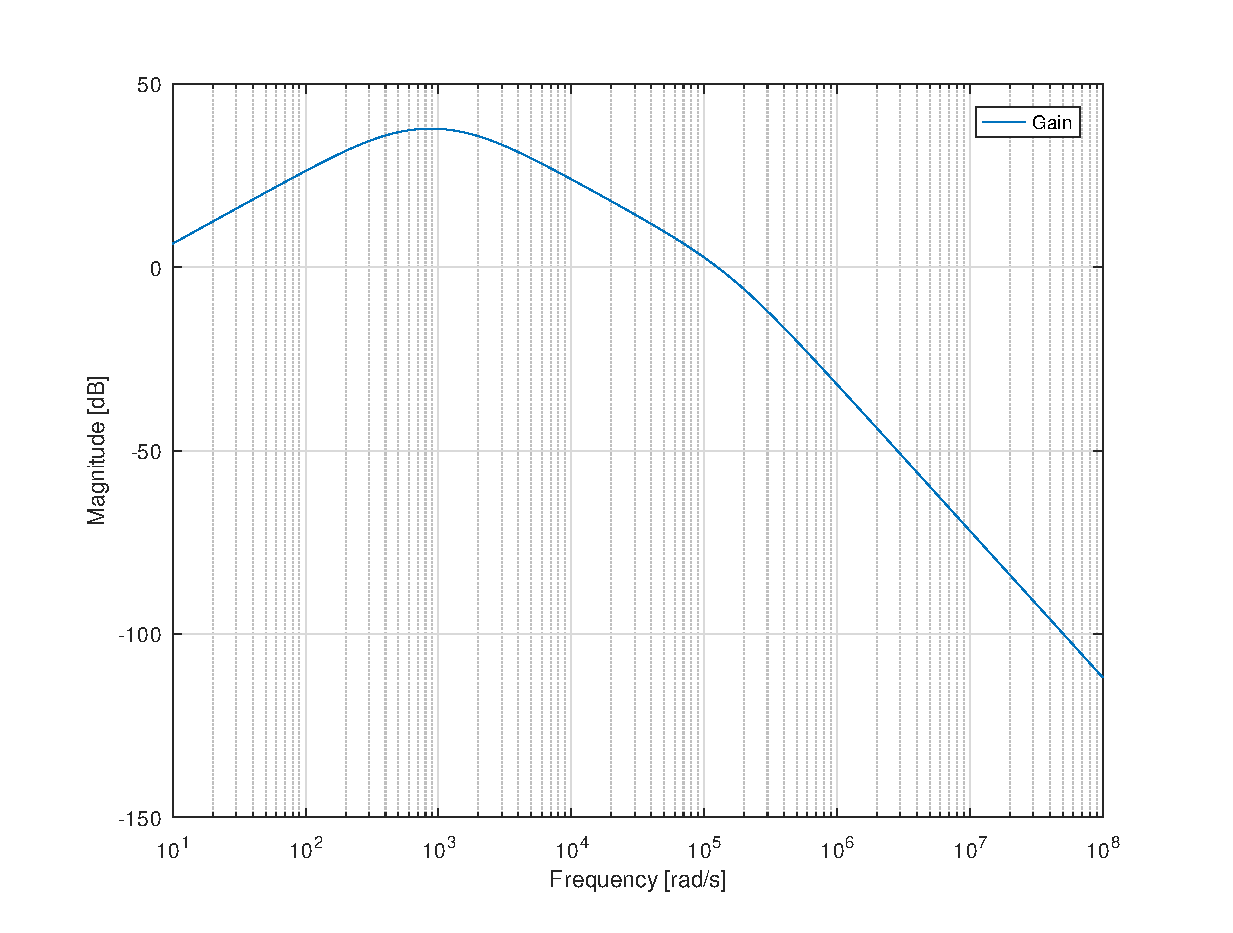
\includegraphics[width=0.6\linewidth]{b3.eps}
\caption{Frequency response: magnitude}
\label{fig:rc2}
\end{figure} 

\begin{figure}[H] \centering
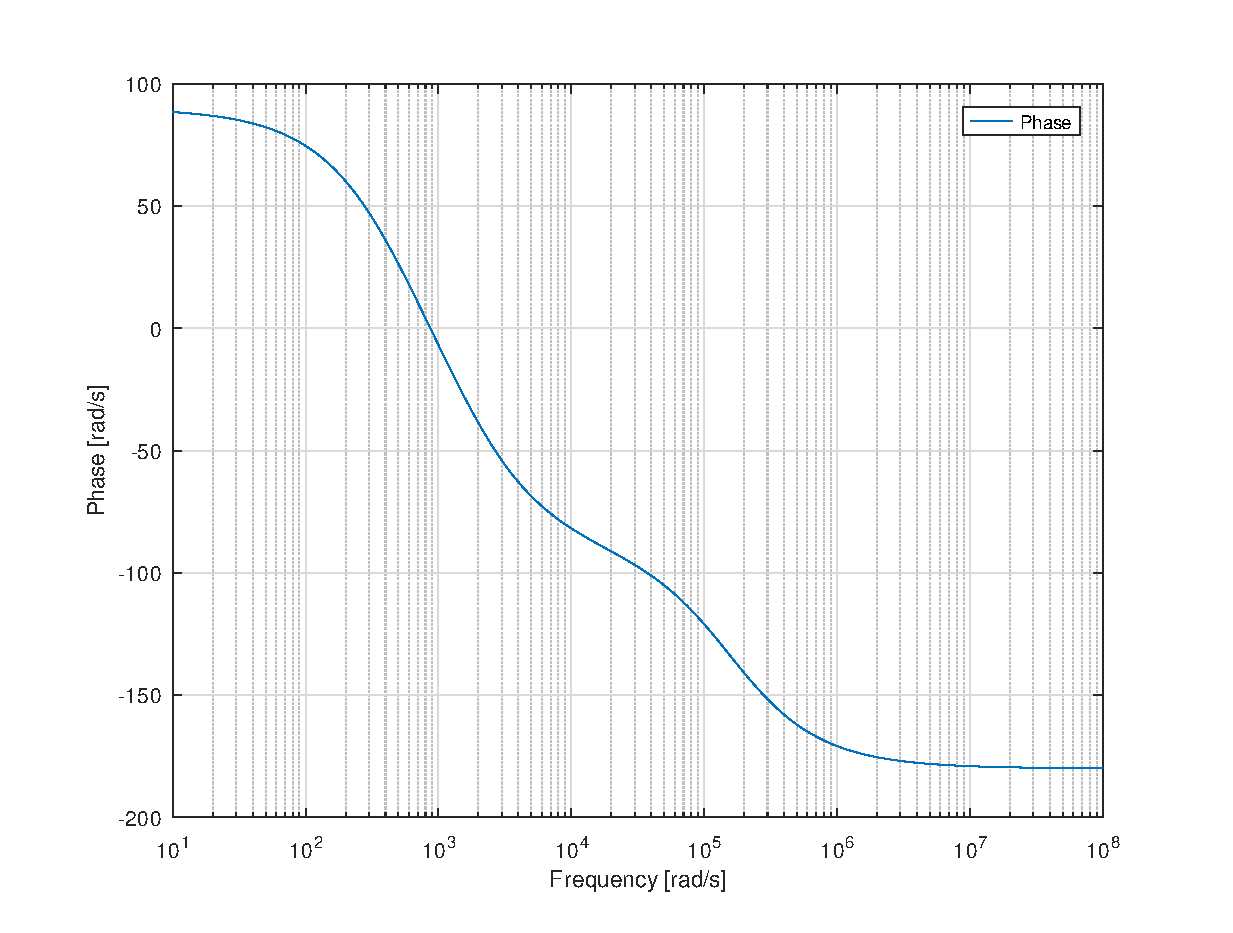
\includegraphics[width=0.6\linewidth]{b4.eps}
\caption{Frequency response: phase}
\label{fig:rc2}
\end{figure} 


\newpage

